% to choose your degree
% please un-comment just one of the following
\documentclass[bsc,frontabs,twoside,singlespacing,parskip,deptreport]{infthesis}     % for BSc, BEng etc.
% \documentclass[minf,frontabs,twoside,singlespacing,parskip,deptreport]{infthesis}  % for MInf

\usepackage{graphicx}
\usepackage{wrapfig}
\usepackage{amsmath}
\usepackage{float}
\usepackage[round]{natbib}

\graphicspath{ {images/} }

\begin{document}

\title{Distributed shared memory through key-value stores}

\author{Mantas Serapinas}

% to choose your course
% please un-comment just one of the following
\course{Artificial Intelligence and Computer Science}
%\course{Artificial Intelligence and Software Engineering}
%\course{Artificial Intelligence and Mathematics}
%\course{Artificial Intelligence and Psychology }   
%\course{Artificial Intelligence with Psychology }   
%\course{Linguistics and Artificial Intelligence}    
%\course{Computer Science}
%\course{Software Engineering}
%\course{Computer Science and Electronics}    
%\course{Electronics and Software Engineering}    
%\course{Computer Science and Management Science}    
%\course{Computer Science and Mathematics}
%\course{Computer Science and Physics}  
%\course{Computer Science and Statistics}    

% to choose your report type
% please un-comment just one of the following
%\project{Undergraduate Dissertation} % CS&E, E&SE, AI&L
%\project{Undergraduate Thesis} % AI%Psy
\project{4th Year Project Report}

\date{\today}

% TODO: write an abstract

\abstract{
* Still to be written.
}

\maketitle

% TODO: write acknowledgements

\section*{Acknowledgements}
* Still to be written.

\tableofcontents

%\pagenumbering{arabic}


\chapter{Introduction}

\section{Motivation}

Distributed shared memory (DSM) is memory architecture where physically distributed memory can be accessed as one logically shared address space. Systems based on shared memory architecture reduce the complexity of parallel programming \citep{vodca}. Unfortunately, building an efficient distributed shared memory system is a huge challenge and the documentation on the existing open-source DSMs is rather limited. Thus it can be a daunting task to run parallel programs on distributed shared memory systems.

However, with cloud computing becoming increasingly popular new solution became available, namely NoSQL data stores \citep{nosql-data-stores}. NoSQL can be completely schema-free, most popular data models being key-value stores, document stores, column-family stores, and graph databases. It is able to scale horizontally over many commodity servers. On top of that, some cloud data management systems provide strong consistency model, which means that after update operations all nodes agree on the new value before making it available to the user. All these properties make it possible to use such data stores as distributed shared memory.

The focus of this project is to expose the distributed shared memory model in a cloud by implementing an instrumentation tool which translates load and store instructions to get and put calls to key-value store. This tool will let users to run parallel programs on cloud using key-value store without editing a single line of code.

\section{Scope}

The initial goal of the project was to create the tool which can instrument programs written in any user preferred language but due to communication with Google data store (using gRPC and protocol buffers) a separate gRPC library for each language is needed. The task is trivial but in order to meet the project deadline a single language was chosen, namely C++.

 %TODO_LATER: try with other languages

\section{Approach}

The first phase of the project was about choosing an appropriate key-value store. Google data stores were selected for further benchmarking as they are well documented and widely used in the industry. As Bigtable both showed the best results in throughput and latency, and provides strong consistency, it was chosen to be used as the representative data store for the project. 

%TODO_LATER: the above paragraph needs fixing

The translation of load and store instructions were implemented by writing an LLVM pass. The pass iterates over the instructions and changes load and store instructions to get and put function calls to data store, respectively. Moreover, a new malloc function was created in order to preserve the user program from allocating heap memory for objects, which are stored in Bigtable.

\section{Contributions}

The contributions of this paper are as follows:
\begin{itemize}
\item
Research was done on Google data stores, namely Bigtable, Datastore and Spanner, their features and the consistency models they provide.
\item
Benchmarking the above data stores based on their throughput and latency using YCSB tool.
% \item
% Research on OpenSHMEM and POSIX threads and their suitability for the project (hardware/software required).
\item
Research on possible ways to translate load and store instructions (Intel PIN, LLVM).
\item
Implementing an LLVM pass to do the translation and linking it with gRPC, protobuf and googleapis libraries to communicate with Bigtable instance table.
\item
Implementing a malloc() function to preserve the user program from allocating heap memory for objects.
\end{itemize}

% TODO_LATER: update contributions

\section{Synopsis}

Chapter 2 presents the main requirements for the data stores to be used as distributed shared memory systems. The chapter continues with the background information on the selected Google Cloud data stores, namely Bigtable, Datastore and Spanner. Finally, the chapter discusses the results of the benchmark ran on these data stores.

Chapter 3 starts with the architecture of the tool, also briefly introducing gRPC and protobuf libraries. Then, the chapter briefly talks about the unsuccessful attempt to translate store and load instructions to get and put operations on data store using Intel PIN tool. The chapter continues with an LLVM pass implementation.

Chapter 4 presents the memory wasting problem, introduced by storing heap variables on Bigtable, and describes the solution - the implementation of custom heap memory allocation functions. 

Chapter 5 discusses the correctness and efficiency of the system. 

Chapter 6 introduces the API which lets computers on two different locations in the world use the key-value store as distributed shared memory in scenarios like producer/consumer.

Chapter 7 summarizes the work done and possible ways of improving the system.

\chapter{Data store for DSM}

\section{Overview}

In order to build and test the translation tool, a single cloud data store was chosen to be used as a distributed shared memory system for the project. The main requirements for the data store were:

\begin{itemize}
\item
provide efficient throughput and latency results;
\item
provide strong consistency model;
\item
have a way to run user programs on the same data centre, the data store is located on;
\item
provide an API to communicate in C++;
\item
preferably provide key-value database model.
\end{itemize}

Three Google cloud storages, which met almost all of the requirements, were suggested, namely Bigtable, Datastore and Spanner. Even though neither of the three candidates had key-value store as their primary database model, they were one of the few that provided communication between C++ program and a data store. Google cloud products provide this functionality through gRPC (open source remote procedure call system) using protobuf library and Google APIs. Moreover, all of these Google data storages can be chosen to be located in the same data centre for best throughput and latency results. Further sections provide a brief look into each of the candidates and show the results of the benchmarking on throughput and latency.

\section{Bigtable}

Bigtable \citep{google-bigtable} is high performance, wide column NoSQL database, which stores data in massively scalable tables, each of which is a sorted key/value map. Tables consists of rows, each of which is essentially a collection of key/value entries, where the key is a combination of the column family, column qualifier and timestamp. 

Bigtable treats all data as raw byte strings. If a row does not include a value for a specific key, the key/value pair simply does not exist. Changes to a row take up extra storage space, as Bigtable stores mutations sequentially and compacts them only periodically, but as the usual amount of data sent from our tool does not exceed 32/64 bits (depending on the machine architecture) the additional amount of memory used is insignificant. 

Most importantly, Bigtable supports look up value associated with key operation and provides strong consistency - all writes are seen in the same order.

\section{Datastore}

Datastore \citep{google-datastore} is highly-scalable NoSQL, document store model database developed by Google. Unlike Bigtable, it provides a SQL-like query language (GQL) and ACID (Atomicity, Consistency, Isolation, Durability) properties for atomic transactions. Moreover, it supports a variety of data types, including integers, floating-point numbers and many more, although such functionality is not needed for purpose of the project as the tool stores binary data directly. Datastore uses synchronous replication, meaning that data is written to primary storage and the replica simultaneously.

Similarly to Bigtable, Datastore provides strong consistency for entity (row) lookups by key. It also provides strong consistency for ancestor queries but they are not relevant to the project.

\section{Spanner}

Spanner \citep{google-spanner} is a horizontally scalable, globally consistent relational database service. Unlike the previously discussed storages, Spanner has an key-value store as additional database model, data scheme and uses SQL. Similarly to the Datastore, it provides ACID transaction properties.

Spanner provides even stronger consistency property than strong consistency, namely external consistency. External consistency guarantees that for any two transactions, T\textsubscript{1} and T\textsubscript{2}: if T\textsubscript{2} starts to commit after T\textsubscript{1} finishes committing, then the timestamp for T\textsubscript{2} is greater than the timestamp for T\textsubscript{1} . 

\section{Benchmarking results}

For the benchmarking an existing industry tool was used - Yahoo! Cloud
Serving Benchmark (YCSB) \citep{ycsb}. A key feature of YCSB, as described by its developers, is that it is extensible. YCSB is open-source, supports easy definitions of new systems and workloads. Workloads allow to understand the performance tradeoffs of different systems.

The main operations done by the translation tool are reads and writes with a small amount of read-modify-write operations on heap allocation pointer, keeping track of the address to next free memory space. Thus, workloads A and F were chosen, simulating update heavy and read-modify-write using systems, respectively.

For the best results the benchmarking was run on Google Compute Engine (GCE) virtual machine situated at the same data centre as the data stores.

\subsection{Loading the data}

Before running the benchmark on workloads, 1000 rows were inserted into each data store. Figures \ref{load-latency} and \ref{load-throughput} show the latency and throughput achieved by each cloud storage. The results show that both Bigtable and Spanner have much lower latency and higher throughput than Datastore. This can be explained by research results on Datastore using synchronous replication, which makes the host wait until all replications are created, as described in Margaret's Rouse article Synchronous replication \citep{synchronous-replication}.

\begin{figure}[ht]
	\centering
	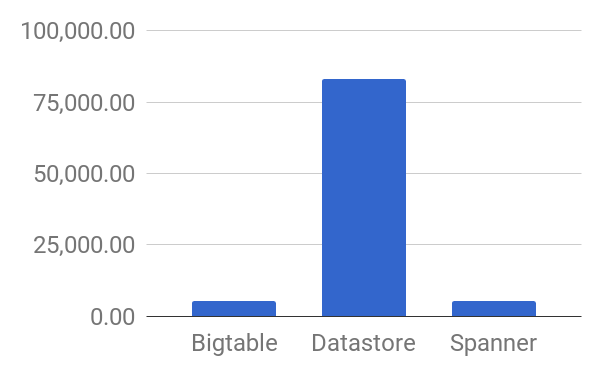
\includegraphics[width=10cm]{load-latency}
	\caption{Latency (\( \mu s\)) for 1000 insert (write) operations}
	\label{load-latency}
\end{figure}
\begin{figure}[ht]
	\centering
	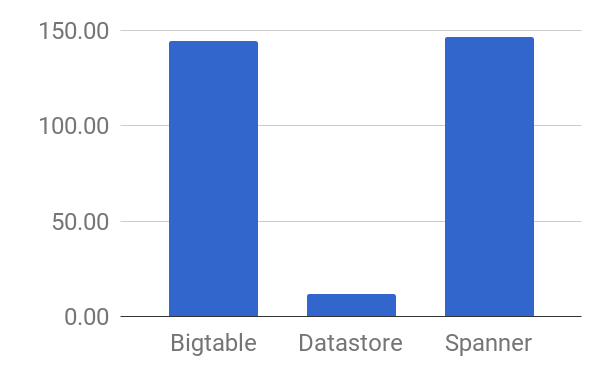
\includegraphics[width=10cm]{load-throughput}
	\caption{Throughput (\(ops/sec\)) for 1000 insert (write) operations}
	\label{load-throughput}
\end{figure}

\subsection{Workloads}

Workload A consists of 1000 operations (500 reads and 500 writes) while workload F consists of 2000 operations (1000 reads, 500 atomic read-modify-write operations and 500 writes). The results of the benchmark in terms of latency on write operations were consistent with the previous loading benchmark results, with Bigtable and Spanner performing significantly better over Datastore (Figure \ref{write-latency}). The latency on write operations showed a clear dominance by Bigtable. 

\begin{wrapfigure}{r}{0.5\textwidth}
	\centering
	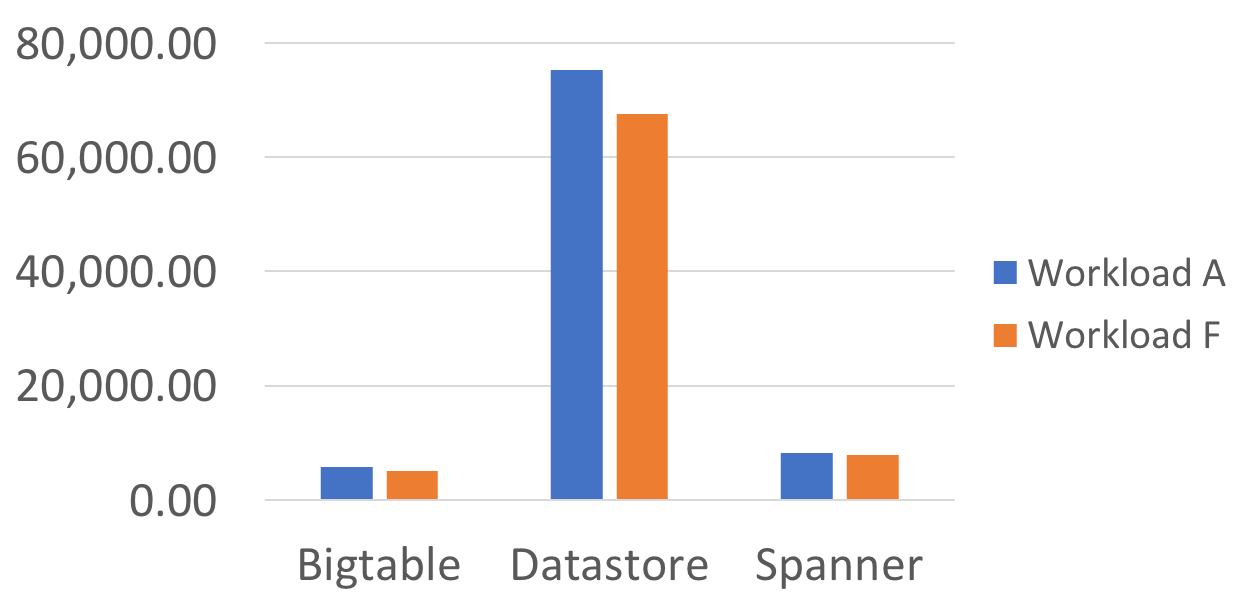
\includegraphics[width=7cm]{write-latency}
	\caption{}
% 	\caption{Write operations latency (\( \mu s\)) for Workload A (500 writes) and Workload B (1000 writes)}
	\label{write-latency}
\end{wrapfigure}

Even though, the difference on read operations latency between Datastore and two other data storages were smaller than with write operations (Figure \ref{read-latency}), Datastore still was more than two times slower than Spanner and more than 4 times slower than Bigtable. The latency results on read-modify-write operations showed a similar trend as read and write operations (Figure \ref{read-modify-write-latency}). 

The overall throughput, again, showed a significant superiority by Bigtable, as indicated in Figure \ref{throughput}. 


\begin{figure}[ht]
	\centering
	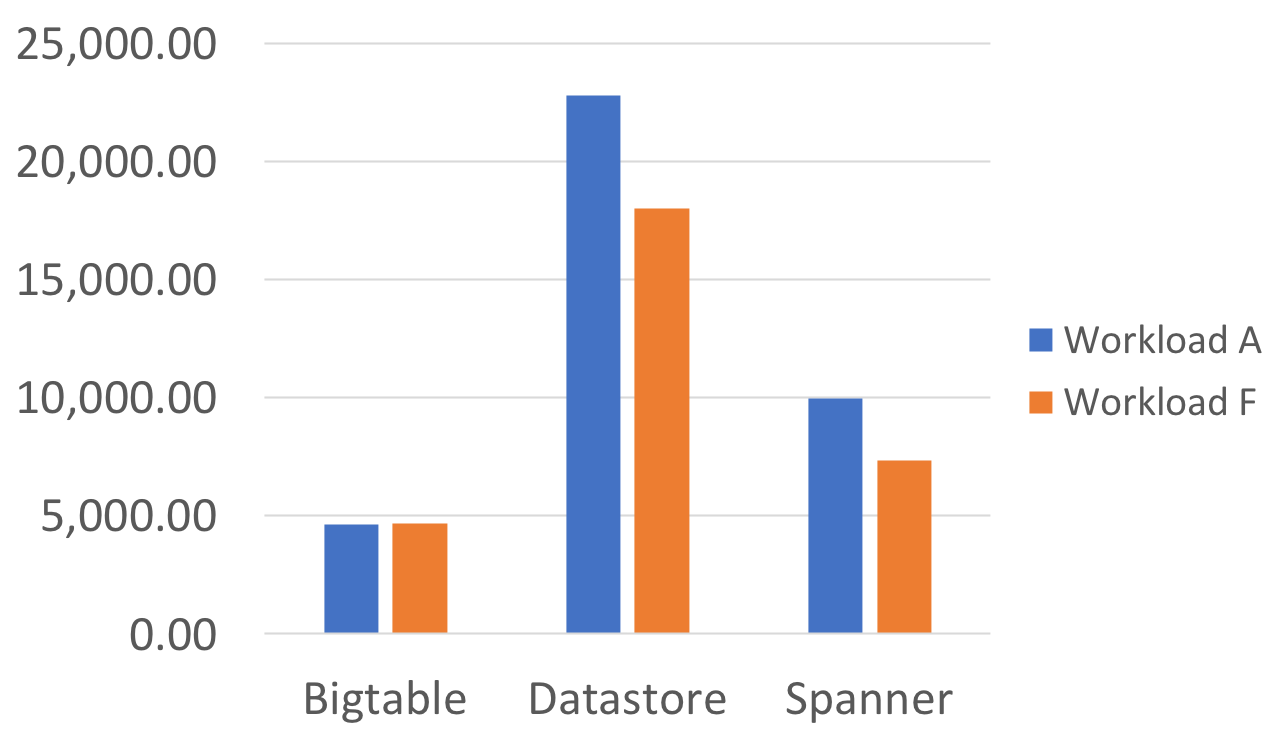
\includegraphics[width=12cm]{read-latency}
	\caption{Read operations latency (\( \mu s\)) for Workload A (500 reads) and Workload B (1000 reads)}
	\label{read-latency}
\end{figure}

\begin{figure}[ht]
	\centering
	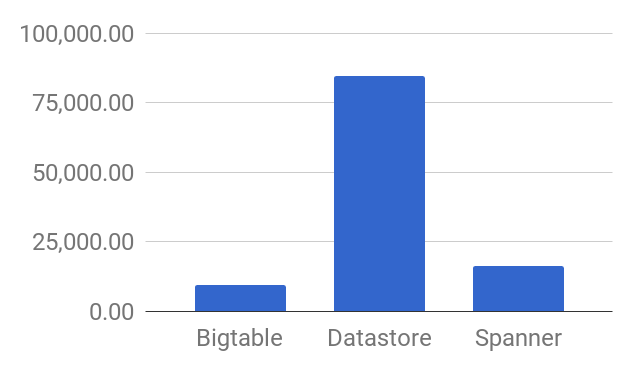
\includegraphics[width=13cm]{read-modify-write-latency}
	\caption{Read-modify-operations latency (\( \mu s\))}
	\label{read-modify-write-latency}
\end{figure}

\begin{figure}[!ht]
	\centering
	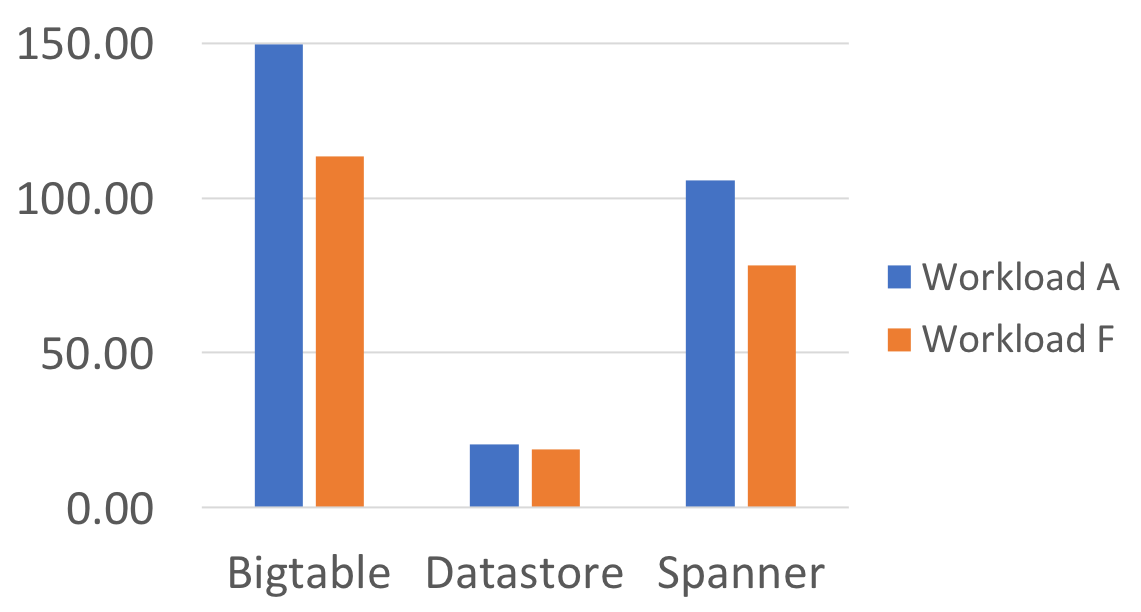
\includegraphics[width=12cm]{throughput}
	\caption{Throughput (\(ops/sec\)) for Workloads A (1000 operations) and Workload B (2000 operations)}
	\label{throughput}
\end{figure}

\subsection{Conclusions}

As Bigtable showed the best results in loading of data and on both of the workloads the benchmarks were run on, and since it provided a strong consistency model, it was selected to be used as a distributed shared memory system for the translation tool.

% FOR INTERIM REPORT  - - - - - - - - - TO BE REMOVED 

\chapter{Interim report}

\section{Accomplishments so far}

\begin{itemize}
\item
Research was done on Google data stores. Benchmarked the above data stores based on their throughput and latency using YCSB tool.
\item
Research was done on OpenSHMEM and POSIX threads and their suitability for the project (hardware/software required).
\item
Research was done on possible ways to translate load and store instructions (Intel PIN, LLVM).
\item
Implemented an LLVM pass to call an external functions (dummy get/put) as the Proof of Concept (PoC) application. Found out how to link gRPC, protobuf and googleapis libraries to create external get/put functions. Implemented the get/put functions for simple static and stack variables storage on Bigtable.
\end{itemize}

\section{Remains to be done}

\begin{itemize}
\item
Create get/put functions to store heap variables, pointers, pointers-to-pointers, etc. Test it!
\item
Heap allocation functions implementation and LLVM pass modification to change the calls from the original heap allocation functions (malloc, calloc, etc) to calls to the implemented ones. Test it!
\item
Create an API which would let imitate the producer-consumer relationship through DSM, with producer and consumer situated in geographically different locations. Bigtable multi regional locations could be used (https://cloud.google.com/storage/docs/bucket-locations\#location-mr).
\end{itemize}

Other possible work is to be determined with project supervisor.

\section{Timeline for final semester}

\begin{tabular} { | c | c | }
	\hline
 		Task & Deadline \\ [0.5ex] 
	\hline
	\hline
	Create get/put functions to store heap variables, pointers, etc. & 1 Feb \\
	\hline
	Implementation of custom heap allocation functions and related subtasks & 10 Feb \\
	\hline
	Create an API & 18 Feb \\
	\hline
	Other tasks (TBD) & 4 Mar \\
	\hline
	Report writing & 5 April \\
	\hline
\end{tabular}

% FOR INTERIM REPORT  - - - - - - - - - TO BE REMOVED 

% \chapter{OpenSHMEM vs POSIX threads}

% \section{Overview}

% \section{OpenSHMEM API}

% \section{POSIX threads}

\chapter{Load and store instructions translation}

\section{Architecture}

\subsection{Overview}

\subsection{gRPC and protobuf}

\subsection{get() and put() functions}

\subsection{Memory management}

\section{Try at Intel PIN}

\section{LLVM pass}

\subsection{Overview}

\subsection{Translation}

\chapter{Problems with heap allocation}

\section{Overview}

\section{Implementation of malloc()}


\chapter{Results}

\chapter{API}

\chapter{Conclusions}

\subsection{Overview}

\subsection{Future work}


% use the following and \citep{} as above if you use BibTeX
% otherwise generate bibtem entries
\bibliographystyle{plainnat}
\bibliography{mybibfile}

\end{document}
